\secnumberlesssection{INTRODUCTION} \label{sec:introduction}
For much of the first half of the last century, it was believed that there were just three fundamental particles: protons, neutrons and electrons.
These three particles however were only able to describe a small portion of the phenomena that defines particles physics, and improvements in particle accelerator and detector technologies gave way to the discovery of a plethora of new particles.
This led to a richer understanding of particle physics and to a simple, unified theory to explain these particles on a fundamental level.

This unified theory eventually became known as the Standard Model of Particle Physics, and it explained the known particles with incredible accuracy.
The theory describes two fundamental types of particles: \textbf{fermions} and \textbf{bosons}.
\textbf{Fermions} make up all the ``stuff'' in the world, and \textbf{bosons} describe the way fermions interact with one another.
\textbf{Fermions} are then further divided into \textbf{quarks}, which make up protons and neutrons, and \textbf{leptons}, which include electrons in addition to more elusive particles like muons, taus and neutrinos~\cite{perkins2000introduction}.

While the Standard Model could predict the properties of particles with incredible precision, it faced one major problem: it could not explain why particles have mass, and thus could not predict the masses of individual particles.
To solve this problem, \cite{higgs1964broken} theorized an extension to the Standard Model, which involved the existence of another fundamental field which gives mass to all fundamental particles.
To prove the existence of this field, a particle that could only come to be from the excitation of this field had to be observed: the famed \textbf{Higgs Boson}.

This particle remained a theory for nearly fifty years, until the European Organization for Nuclear Research (CERN) confirmed that the elusive particle had been observed in $2012$~\cite{aad2012observation, collaboration2008cms}.
This observation was achieved by analyzing the particles produced in the collision of a beam of particles and a target, which is commonly named event in the field of High Energy Physics (HEP).
The experiment was performed in the Large Hadron Collider (LHC) at CERN, which is a type of particle accelerator.
The process of figuring out what particles in which conditions cause each detection or hit is called \textbf{event reconstruction}~\cite{leduff2005longitudinal}, and is usually done in software due to the complexity of analyzing the large amounts of available data~\cite{demchenko2013addressing}.

To reconstruct an event from the available data, it is required to use both an understanding of the physics behind it and a plethora of mathematical tools to estimate the particles' characteristics and trajectories.
Naturally, this process relies on the heavy use of many different hardware components to detect and categorize all the gathered data and of computing units to filter it and reconstruct the event.
Thus, valuable information is obtained that can be used by physicists to further understand the underlying structure of the universe~\cite{sirunyan2017particle}.
An example of a common process the data goes through from the detector to the physics analysis can be seen in figure \ref{fig:data_processing}.

    \begin{figure}[ht]
        \centering
        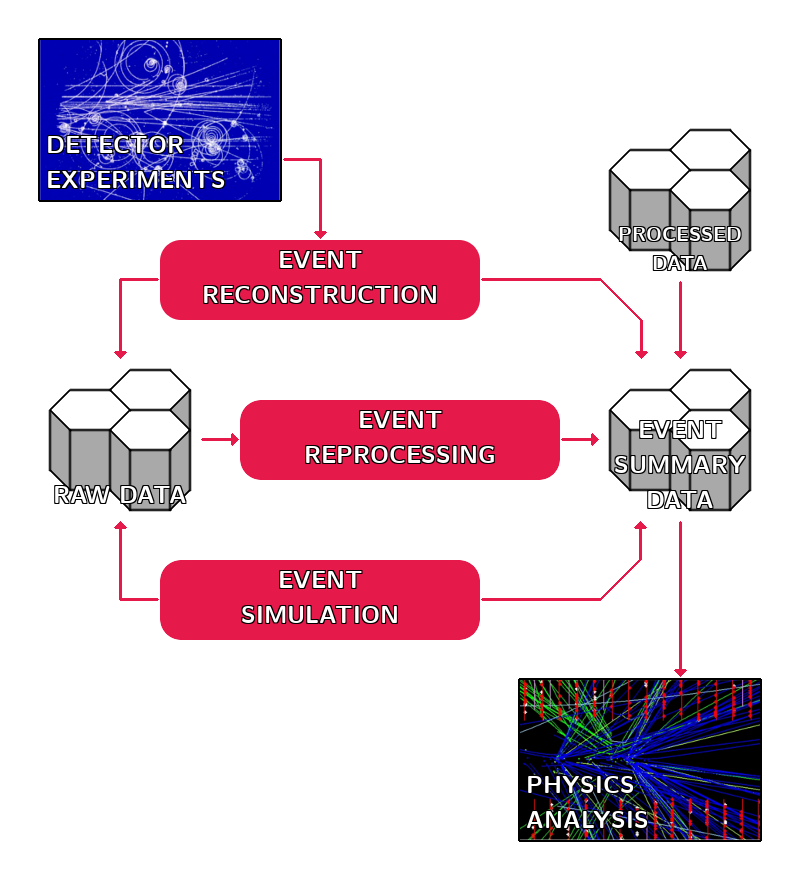
\includegraphics[scale=0.465]{data_processing}
        \caption{\label{fig:data_processing} Example data process found in particle detector software. Source: Own elaboration. Images used are freely available at \texttt{https://home.cern/}.}
    \end{figure}

A common problem that arises from this structure is the fact that, as technology progresses and particle detectors become more advanced, the produced data becomes more detailed and thus more expensive to process.
This issue is seen too at the Thomas Jefferson National Accelerator Facility (TJNAF) in Virginia, USA, where the linear accelerator and its paired detectors produce large amounts of data faster than what the available hardware can cope with. % Note: While this could use a citation, it only rises from conversations with Veronique and Vardan and afaik there ain't any formal documents regarding the issue.
Two natural solutions can be seen to this problem: Upscale the hardware to deal with the ever-increasing amounts of data to be processed; or improve the software to process more information without using new resources.
While the first option can't always be avoided, it's easy to see that the second is usually preferable since it helps alleviate the expenses of upgrading hardware.
In the present document, this second solution is explored by thoroughly going through each factor that slows down the data processing speed and assessing them separately.

% \newpage

% AREA IN COMPUTER SCIENCE/ENGINEERING
While the problem analyzed in this document belongs to the field of High Energy Physics, the effort done is more closely related to algorithms and complexity analysis.
This is attributed to the fact that the nature of the work lies in the underlying framework of the event reconstruction process, which in its core is about minimizing the error in a fit.
This by no means is a problem unique to physics.
Due to this, the contribution of this work has multiple objectives: It directly benefits the software development team at TJNAF in that it accelerates the software used, and it also provides a framework for other projects that look into speeding up the computation of the event reconstruction software for other particle accelerators or systems in general.

% A sample of these contributions would be, for example, the possibility of using mathematical tools for working with matrices such as the Sherman-Morrison formula, the matrix determinant lemma or the Cholesky decomposition for speeding up the update phase of an Extended Kalman Filter (EKF), described in Section \ref{ssec:prop_matrices}.

% The improvement in the processing time of the software brought by each step of the solution applied in this work can be seen in Figure \ref{fig:engines_times_improvements}.
% DCHB and DCTB are the engines used in the reconstruction software where this project's work is focused.

%     \begin{figure}[ht]
%         \centering
%         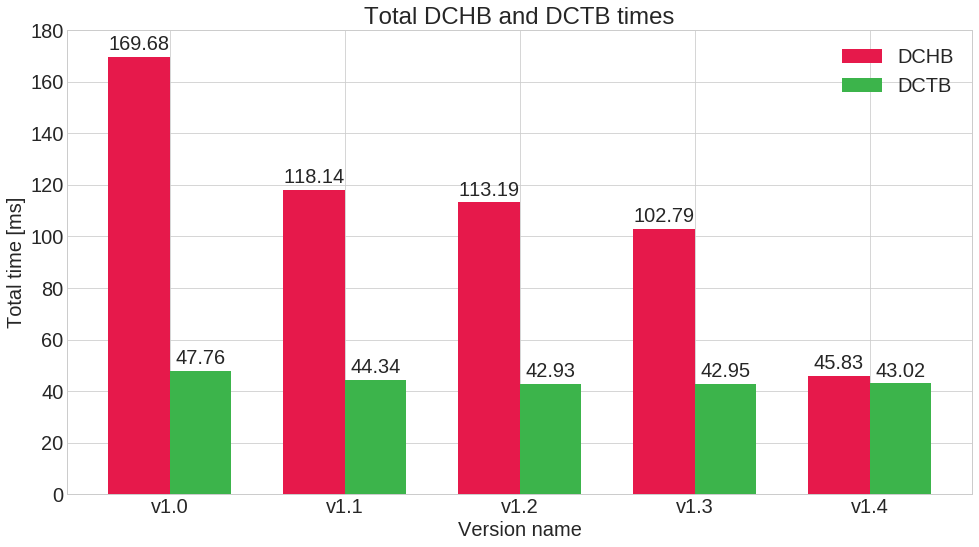
\includegraphics[scale=0.44]{engine_times/complete_improvement}
%         \caption{\label{fig:engines_times_improvements} Engine time improvements for DCHB and DCTB over the different versions. Source: own elaboration.}
%     \end{figure}

% \newpage

Figure \ref{fig:clas12_software_diagram} shows a detailed tree diagram of the CLAS12 software components.
CLAS12 is the reconstruction software used at TJNAF, and is described in detail in Section \ref{ssec:framework_clas12}.

    \begin{figure}[ht]
        \centering
        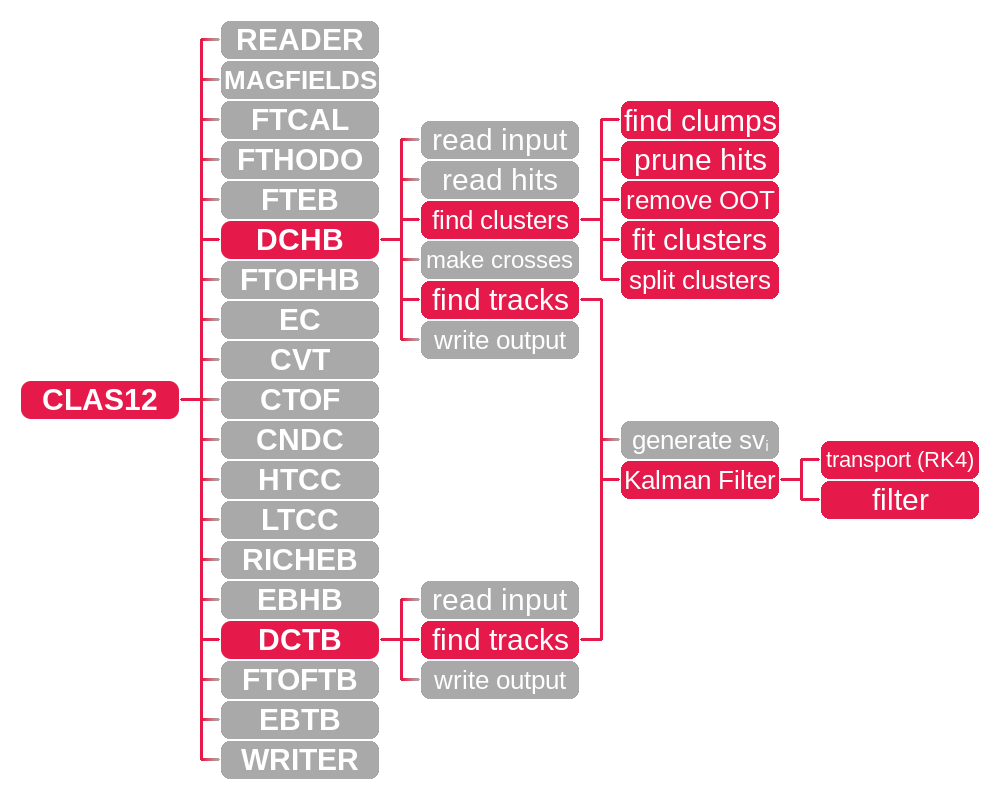
\includegraphics[scale=0.44]{clas12_software_diagram}
        \caption{\label{fig:clas12_software_diagram} Tree diagram with the CLAS12 software components. The components where the project's work is focused are highlighted.}
    \end{figure}

\newpage

Chapter $1$ presents a part of the current state of the art, along with a short description of each publication listed.
In Chapter $2$ the problem is formally defined, along with its context and the goals of the project.
In Chapter $3$ most of the large concepts that are related to the project and the document are explained, including the hardware and the software components.
Chapter $4$ elucidates in detail the profiling process described previously and presents the results of the profiling sessions.
Chapter $5$ explains the solutions implemented to each different bottleneck found in Chapter $4$ and proposes an algorithm for future work.
Then in Chapter $6$ the validity of the results produced after each change is asseverated and the computing times are compared.
Finally, Chapter $7$ provides with the concluding remarks of the work, including the setbacks faced and future work is proposed. % CHAPTER REFERENCE